\subsection*{AND-gate}
\label{volumenkontrol-design-and}

De to AND-gates er designet med diskrete komponenter, fremfor en integreret kreds. AND-gaten fungere ved at holde udgangen høj, når begge indgange er høje. På AND-gaten til venstre på figur \ref{fig:volumenkontrol_diagram}, er et højt udgangs niveau ~0,6 V, dette skyldes at der på udgangen af gaten er en transistor, basis-emitter overgang, til stel. Er blot den ene af indgangene lave, vil den trække udgangen til stel gennem den tilhørende diode, BAT85. Databladet for dioden beskriver en sammenhæng mellem en diode spænding på 0,24 V og en strøm gennem den på 0,1 mA, dette resultere i en Pull-up modstand beregnet i ligning (\ref{equ:and-gate1}).

\begin{equation}
\label{equ:and-gate1}
V_{CC} - V_D = R_{15} \cdot I_F = 5~\mathrm{V} - 0,24~\mathrm{V} = R_{15} \cdot 0,1~mA \Rightarrow R_{15} = 47,6~k\ohm
\end{equation}

Udgangen af AND-gaten vil altså ikke kunne bliver højere end 0,24 V, ved lavt output.

\subsection*{Tæller}
\label{volumenkontrol-design-taeller}

\begin{figure}[h]
\centering
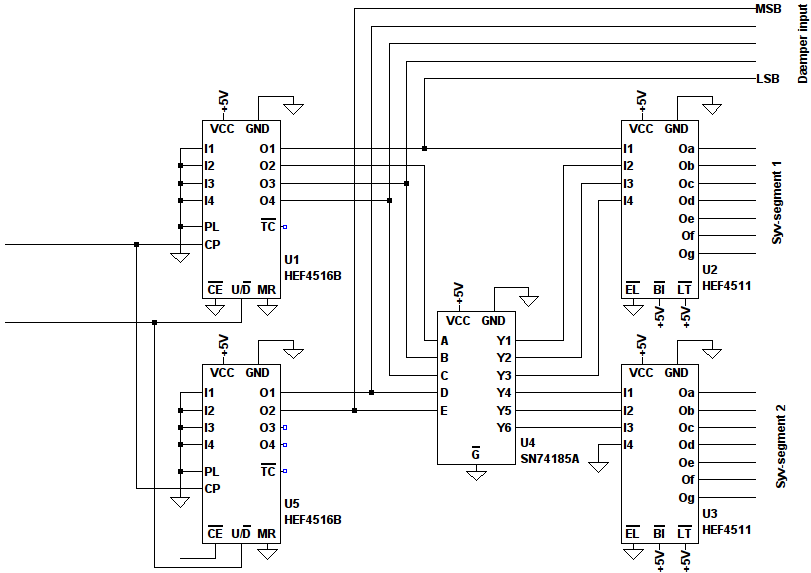
\includegraphics[width=\textwidth]{teknisk/volumenkontrol/taeller.png}
\caption{Diagram over tælleren og displaydriveren}
\label{fig:taeller}
\end{figure}
\fixme{Jonas - Tilføj tællerstyring}
Tællerens opgave er at holde styr på hvad volumenniveauet er og diagrammet for den er vist på figur \ref{fig:taeller}. Der tælles op eller ned når der trykkes på én af de to volumenknapper. Hvor hurtigt der skal tælles, bestemmes af det AND'ede signal fra VCO'en og XOR-gaten. VCO'en fungerer som en clock på AND-gaten, mens XOR-signalet sørger for, at det kun er den ene knap der holdes nede. Hvis begge knapper holdes nede, vil XOR-signalet være lavt, og der vil intet signal blive sendt til tælleren. Om der skal tælles op eller ned, styres af et signal fra den knap der repræsenterer et ønske om en sænkning i volumeniveau. Hvis denne er nede, som den eneste knap, vil tælleren tælle ned af. Hvis denne ikke er nede, men XOR-signalet stadig er højt, betyder det at den anden knap er nede og tælleren vil derfor tælle op. Tælleren giver et binært output, som danner grundlag for hvad der vises i displayet og hvordan reguleringen af volumen indstilles. Tælleren der benyttes er en 4-bit tæller af typen HEF4516B\fixme{kilde: datablad}. Da fire bit ikke er nok skal der bruges to tællere. Yderligere skal der også bruges noget kontrollogik, for at sikre tælleren ikke tæller for højt eller lavt og for at styre den anden tæller.

\subsection*{Display}
\label{volumenkontrol-design-display}
Indstillingen af volumenkontrollen vises på to 7-segmenter. Dette er valgt, fordi disse er enkle at styre med simple kredsløb og det derfor ikke er nødvendigt med en microcontroller for at styre dem, som tilfældet havde været, hvis et LCD-display i stedet var blevet benyttet.

\subsection*{Displaydriver}
\label{volumenkontrol-design-display_driver}
Displaydriveren konverterer signalet fra tælleren til et signal der kan vises på de to 7-segment displays. Der konverteres fra tællerens binære output til BCD, Binary-coded decimal, for så at konvertere det til et signal 7-segment displaysne kan vise. Der benyttes en SN74185A\fixme{kilde: datablad} til konverteringen fra binær til BCD. Fordelen ved at konvertere til BCD først er at denne konvertering også deler det binære tal op i to, en'ere og ti'ere. Disse to binære tal sendes igennem en 7-segmentsdriver, HEF4511\fixme{kilde: datablad}, for at få et output der fungerer med 7-segmenterne. Displaydriveren er også vist på figur \ref{fig:taeller}.

\subsection*{Dæmper}
\label{volumenkontrol-design-daemper}
Dæmperen er en en analog attenuator, som er sammensat af to sæt modstandsattenuatore, hver efterfulgt af en buffer. Dæmpningen indstilles ved at ændre, hvor signalet tages ud af de to modstandsattenuatore, ved brug af en analog multiplekser. Den første attenuator består af syv modstande, hvor der er en dæmpning på 8 dB mellem hver \fixme{hver hvad?}. Den anden attenuatorer består af otte modstande, hvor der er en dæmpning på 1 dB mellem hver\fixme{hver hvad?}. Det er således muligt at kombinere de to attenuatorer til at dæmpe signalet mellem 0 og 55 dB, med et interval på 1 dB. Diagrammet er afbilledet på figur \ref{fig:volumenkontrol_daemper} og modstandene derpå er beregnet i Appendiks C??.

\begin{figure}[h]
\centering
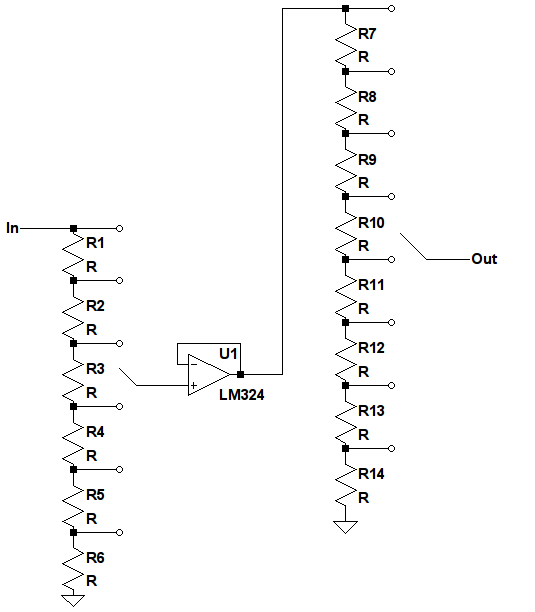
\includegraphics[width=\textwidth]{teknisk/volumenkontrol/daemper.png}
\caption{Diagram over dæmperen}
\label{fig:volumenkontrol_daemper}
\end{figure}

\section{Simulering}
\label{volumenkontrol-simulering}

Som det ses på figur \ref{fig:vco-signal} svinger udgangen på integratoren mellem schmitt-triggerens to niveauer. Det kan også ses udfra grafen hvornår VCO'ens udgang er høj, dette er når integratorens udgang, den blå kurve, er højere end $U_{6_{\mathrm{in+}}}$, den røde kurve.

\begin{figure}[h]
\centering
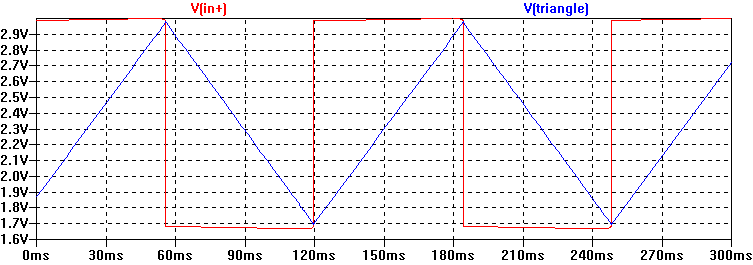
\includegraphics[width=\textwidth]{teknisk/volumenkontrol/vco-signal.png}
\caption{Integratorens udgang og $U_{6_{\mathrm{in+}}}$}
\label{fig:vco-signal}
\end{figure}

\fixme{Jonas - Simulering af konstantstrømsgeneratoren}
\fixme{Jonas - Simulering af Stress test}

\section{Accepttest}
\label{volumenkontrol-accepttest}

